\documentclass[11pt, a4paper, oneside]{article}
\usepackage{worksheet}

\begin{document}
	\author{L. Bung}
	\title{Zylinder}
	\subject{Mathematik}
	\class{2BF1}
	\maketitle
	
	\warning{Merke}{
	Die \textbf{Grundfläche} $G$ eines Zylinders lässt sich errechnen mit $G=\pi \cdot r^2$.
	
	Die Formel für die \textbf{Mantelfläche} $M$ lautet $M = u \cdot h = 2 \cdot \pi \cdot r \cdot h$. 
	
	Das \textbf{Volumen} eines Zylinders ist $V=G \cdot h = \pi \cdot r^2 \cdot h$.
	
	Die \textbf{Oberfläche} eines Zylinders ist $O=2 \cdot G + M = 2 \cdot \pi \cdot r^2 + 2 \cdot \pi \cdot r \cdot h$.}
	
	\singletask{Oberfläche und Volumen von Zylindern}
	
	Berechnen Sie jeweils die Oberfläche und das Volumen der Zylinder.
	
	a) $r = 2$ cm; $h = 6$ cm
	
	\checkered
	
	b)
	\begin{figure}[h!]
		\begin{minipage}{.245\textwidth}
			\centering
			\begin{tikzpicture}
				\tkzDefPoint(1,1){M1}
				\tkzDefPoint(0,1){A}
				\tkzDefPoint(2,1){B}
				\tkzDefPoint(1,4){M2}
				\tkzDefPoint(0,4){C}
				\tkzDefPoint(2,4){D}
				\tkzDrawCircle[black](M2,C)
				\tkzDrawSemiCircle[black](M1,A)
				\tkzDrawSemiCircle[dashed, black](M1,B)
				\tkzDrawLines[add=0 and 0](A,C B,D)
				\tkzDefPoint(2,2){E}
				\tkzLabelPoint[below right, rotate=90](E){$h=4$ cm}
				\tkzDrawLine[dashed, black, add=0 and 0](A,B)
				\tkzDrawPoint(M1)
				\tkzLabelPoint[below](M1){$d=2.5$ cm}
			\end{tikzpicture}
		\end{minipage}
	\begin{minipage}{.75\textwidth}
		\centering
		\checkered[6cm]
	\end{minipage}
	\end{figure}
	
	\pagebreak
	
	\singletask{Konstruktion bei gegebenem Volumen}
	
	Konstruieren Sie einen Zylinder, der ein Volumen von 30 $\text{cm}^3$ hat:
	Geben Sie Radius und Höhe an und zeichnen Sie das Netz mit beschrifteten Längen.
	
	Wie groß ist die Oberfläche Ihres Zylinders?
	
	\checkered[18cm]
	
	\partnertask{Kessel einer Dampflokomotive}
	
	\begin{figure}[h!]
		\centering
		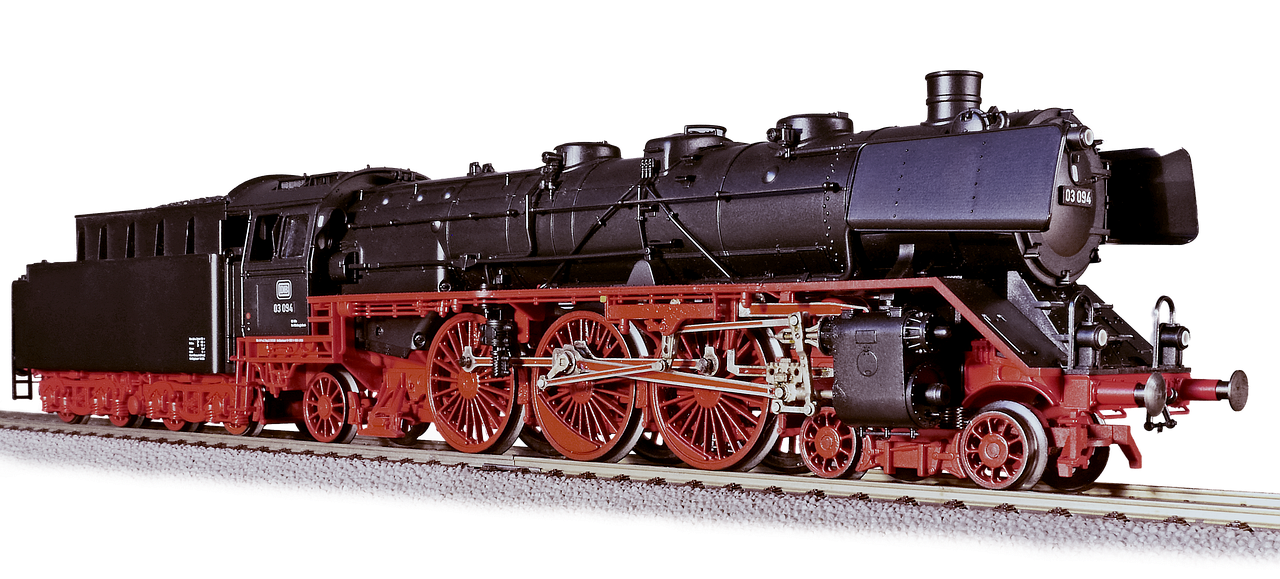
\includegraphics[width=.5\textwidth]{steam-locomotive.png}
	\end{figure}

	Der Kessel einer Dampflokomotive ist 10 Meter lang.
	Die Gesamthöhe der Lok beträgt 7 Meter und die Unterkante des Kessels befindet sich 2 Meter über den Schienen.
	Berechnen Sie das Volumen des Kessels.
	
	\hint{Tipp}{Fertigen Sie zuerst eine Skizze an, in der Sie alle benötigten Maße notieren.}
	
	\checkered[12.5cm]	
\end{document}
